\section{Evaluation}
\label{sec:evaluation}
The evaluation separates control quality, communication cost, and system
timing. The principal control results use $\pi_{0.5}$ in simulation;
OpenVLA-OFT provides a second visual interface with less complete baseline
coverage. The hardware deployment uses recorded SO-101 observations
replayed through the real client and cloud stack. Physical closed-loop
task success has not yet been measured in this deployment.

\subsection{Setup and Statistical Protocol}
\paragraph{Benchmarks.}
LIBERO~\cite{libero} evaluation covers the Spatial, Object, Goal, and Long
suites, with ten evaluated tasks and 50 episodes per task in each suite,
for 2,000 episodes per method. The primary $\pi_{0.5}$ comparisons use
the same A40 host and evaluation framework. The two camera streams are
encoded together for payload accounting, and a new observation is uploaded
every five control steps.

RoboCasa365~\cite{robocasa365} evaluation covers 24 atomic tasks with
three cameras. The initial batch contains 20 episodes per task, for 480
episodes, under the recorded 1.5-times task-time-limit setting. The
training-domain input protocol renders at 256 resolution, applies the
AV1 processing associated with the training data, and produces the
224-resolution policy input. The reference retains this preprocessing
without additional transport compression. It is consequently distinct
from native 224 rendering or unprocessed 256 rendering. We report a
second 480-episode batch separately when combining reference and proposed
method outcomes.

\paragraph{Baselines.}
The image paths include the reference input, JPEG, streaming H.264, and
SPARC~\cite{sparc}. The LIBERO H.264 configuration uses libx264 with
low-latency operation, no B-frames, and GOP 16. We report both CRF 30 and
CRF 23 instead of interpreting one bitrate as a complete codec
rate--quality curve. The SPARC LIBERO checkpoint is trained for the
associated policy. OFT baseline coverage is incomplete, so transferred
checkpoints from a different policy are not used as evidence of a fair
compression advantage.

\paragraph{Metrics and uncertainty.}
We report episode success counts, success-rate differences in percentage
points, and paired 95\% confidence intervals. The statistical
analysis uses Newcombe paired intervals and exact two-sided McNemar
tests on discordant outcomes. Initial conditions and evaluation hosts are
matched within comparisons. Matching initial conditions does not imply
identical policy randomness: RoboCasa's reference, SPARC, and H.264
clients shared a policy service, whose random-number sequence was not
aligned invocation by invocation.

A confidence interval containing zero is not evidence of equivalence.
The exploratory noninferiority thresholds in the existing analysis were
selected after observing results, and we do not use them as a
preregistered guarantee. Payload samples, episode outcomes, and upload
latencies also have different denominators and are identified separately.

\subsection{Control Quality and Payload}
\paragraph{LIBERO.}
Table~\ref{tab:libero} gives success counts by suite. The proposed
configuration succeeded in 1,934 of 2,000 episodes, compared with 1,938 for
the reference. The paired difference was $-0.20$ percentage points with a
95\% interval of $[-1.21,0.81]$ and $p=0.767$. Figure~\ref{fig:paired}
places this difference alongside those of the image baselines.

\begin{table}[t]
\caption{$\pi_{0.5}$ on LIBERO. Each suite has 500 episodes.
Payloads cover both cameras; the proposed method's measured rANS
payload comes from a separate deployment subset, not the full
2,000-episode success run. Image-codec payloads follow the run summaries.}
\label{tab:libero}
\centering\small
\setlength{\tabcolsep}{3.5pt}
\begin{tabular}{lrrrrr}
\toprule
Method & Spatial & Object & Goal & Long & Total \\
\midrule
Reference & 495 & 491 & 486 & 466 & 1,938 \\
H.264 CRF 30 & 487 & 494 & 485 & 450 & 1,916 \\
H.264 CRF 23 & 494 & 492 & 480 & 461 & 1,927 \\
SPARC & 493 & 492 & 478 & 459 & 1,922 \\
Ours & 492 & 492 & 485 & 465 & 1,934 \\
\bottomrule
\end{tabular}
\par\smallskip
\begin{tabular}{lrrrr}
\toprule
Method & H.264/30 & H.264/23 & SPARC & Ours \\
\midrule
Mean payload (kB) & 1.74 & 3.50 & 0.37 & 1.82 \\
\bottomrule
\end{tabular}
\end{table}

\begin{figure}[t]
\centering
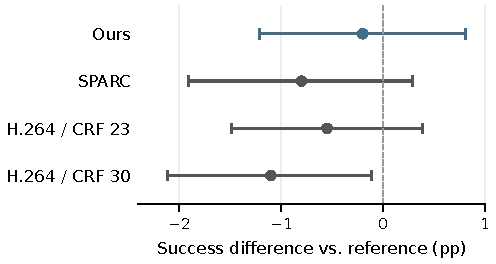
\includegraphics[width=\columnwidth]{images/libero-paired-differences.pdf}
\caption{Paired success-rate differences from the LIBERO reference.
Intervals are paired 95\% confidence intervals; they are not inferred
from independent binomial samples.}
\Description{A horizontal interval plot compares the proposed method,
SPARC, and two H.264 settings with the reference. The proposed method
has a difference of minus 0.20 percentage points with an interval
from minus 1.21 to plus 0.81.}
\label{fig:paired}
\end{figure}

SPARC had the smallest reported payload in this comparison. Our direct
success-rate difference from SPARC was $+0.60$ percentage points
($[-0.45,1.66]$, $p=0.299$). H.264 CRF 30 is below the reference by
$1.10$ percentage points ($[-2.11,-0.11]$, $p=0.035$), but the direct
comparison between our method and that H.264 setting is not significant.
The difference is $+0.90$ percentage points, with a 95\% interval of
$[-0.16,1.97]$ and $p=0.111$.
The stronger H.264 CRF 23 setting succeeded in 1,927 episodes at a larger
payload. These points characterize available operating configurations;
they do not establish a minimum bitrate required by either method.

Actual rANS deployment was checked on a separate 200-episode subset,
with 50 episodes per suite. Mean payloads were 1,857, 1,599, 2,035, and
1,787 bytes for Spatial, Object, Goal, and Long, respectively, giving
approximately 1.82\,kB per upload. The entropy path recovered the
quantized codes losslessly. Rerunning a policy can nevertheless change
individual episode outcomes, so coding correctness is distinguished
from rollout determinism.

\paragraph{RoboCasa input-domain sensitivity.}
Table~\ref{tab:robocasa} reports the first training-domain batch. The
reference succeeded in 291 episodes and the proposed configuration in
295, with a paired difference of $+0.83$ percentage points
($[-3.93,5.59]$, $p=0.797$). The second batch yielded 286 versus 275.
Pooling the two within-batch comparisons gives 577 reference successes
and 570 proposed-method successes in 960 episodes, a difference of
approximately $-0.7$ percentage points ($[-4.1,2.7]$, $p=0.72$).
The width of this interval prevents a narrow claim about preserved
performance.

\begin{table}[t]
\caption{First RoboCasa training-domain batch, 480 episodes. The
reference includes training-domain AV1 preprocessing but no extra
transport compression. Payloads are the recorded configuration summaries;
complete wire-level accounting is not established by this table.}
\label{tab:robocasa}
\centering\small
\begin{tabular}{lrr}
\toprule
Method & Payload (kB) & Successes \\
\midrule
Training-domain reference & -- & 291 \\
SPARC & 0.97 & 277 \\
H.264 CRF 44 & $\sim$1.1 & 4 \\
H.264 CRF 34 & $\sim$3.0 & 0 \\
Ours, lower rate & 1.14 & 295 \\
Ours, higher rate & 3.0 & 272 \\
\bottomrule
\end{tabular}
\end{table}

The reference itself changes with preprocessing: unprocessed 256
rendering gives 251 successes, and a separate native-224 protocol gives
190. We therefore do not interpret a comparison against the native-224
reference as a compression improvement under the training-domain
protocol. The low-rate H.264 configurations perform poorly in the first
batch, but available results do not establish a single causal source of
that failure or a complete high-rate recovery curve. Similarly, the
higher payload of one learned configuration does not ensure higher
success because these are separately trained operating points.

\subsection{Latency through the Deployed Stack}
The SO-101 latency experiment replays recorded red-block observations
through an Orin client and A40 policy server over the actual link.
Table~\ref{tab:replay} reports complete request quantiles and uses the
task-specific block checkpoint for SPARC. Both its original execution
layout and an all-GPU layout are included. Figure~\ref{fig:replay}
shows the corresponding median and 95th-percentile request times.

\begin{table}[t]
\caption{Recorded-observation replay through the deployed stack.
Each method has 195 uploads after warm-up. Payloads in this table
use KiB ($1\,\mathrm{KiB}=1,024$ bytes); SPARC payloads are in bytes.
These are request measurements, not physical task trials.}
\label{tab:replay}
\centering\small
\begin{tabular}{lrrr}
\toprule
Method & Payload & p50 (ms) & p95 (ms) \\
\midrule
Raw & 220.5 KiB & 397.1 & 815.6 \\
JPEG q90 & 15.2 KiB & 282.3 & 301.1 \\
H.264 CRF 30 & 1.2 KiB & 272.4 & 285.9 \\
SPARC block, original & 742 B & 856.3 & 933.1 \\
SPARC block, GPU & 742 B & 431.3 & 438.0 \\
Ours & 1.3 KiB & 228.4 & 237.5 \\
\bottomrule
\end{tabular}
\end{table}

\begin{figure}[t]
\centering
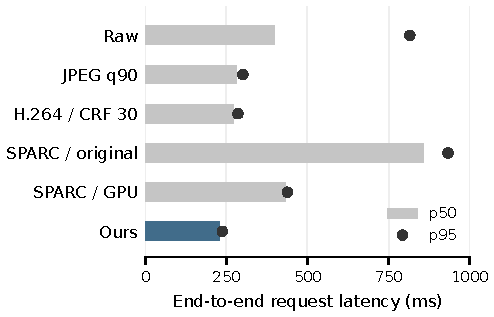
\includegraphics[width=\columnwidth]{images/replay-request-latency.pdf}
\caption{Complete request latency in recorded-observation replay.
Bars show p50 and points show p95; the point is a quantile, not an
uncertainty interval. SPARC uses the block-specific checkpoint.}
\Description{Horizontal latency bars and tail-quantile points for raw
images, JPEG, H.264, two SPARC execution layouts, and the proposed
feature path.}
\label{fig:replay}
\end{figure}

Median latency was 228.4\,ms for the proposed path and 272.4\,ms for
H.264, a reduction of approximately 16.2\% in this deployment.
The task-specific SPARC GPU layout had a smaller payload but a median
of 431.3\,ms. This comparison illustrates why payload and request
latency must be reported together. The ranking is not a result about
all cloud GPUs or networks.

The proposed path's edge median was 13.6\,ms, compared with 2.9\,ms for
H.264; its cloud-total median was 184.3\,ms versus 240.3\,ms. These are
separately aggregated stage measurements and do not add exactly to the
end-to-end medians. They identify the separate edge and cloud costs, while
the complete request duration remains the primary timing metric.
Uploads within a replay sequence are correlated, and no trial-level
confidence claim is derived from treating them as independent tasks.

\subsection{Backbone Adaptation and Component Diagnostics}
The initial OpenVLA-OFT evaluation covered 2,000 episodes, with
1,933 successes versus 1,923 for its reference. Subsequent evaluation
found baseline drift, motivating a contemporaneous rerun. The recorded
partial rerun contains 1,743 versus 1,748 successes in 1,800 episodes.
These windows are not pooled. Until the policy-matched SPARC and image
baselines are complete, this evidence supports interface feasibility
rather than a full cross-backbone compression ranking. The recorded
17.5\,kB OFT rate also requires consistent wire-level validation before
being compared with the primary configuration's sampled rANS payload.

A visual-path microbenchmark records 17.6\,ms for OFT edge encoding
and 10.2\,ms for cloud recovery. Its H.264 comparison includes 2.1\,ms
of edge encoding, 5.3\,ms of decoding, and 39.6\,ms for the original
visual towers. These component measurements use synthetic motion
frames for video decoding and are not a substitute for a complete
same-input deployment comparison.

For $\pi_{0.5}$, a recorded student-tower measurement is 11.0\,ms
versus 39.9\,ms for the original tower. The non-distilled codec variant
succeeds in 1,918 LIBERO episodes versus 1,934 for the main configuration.
This diagnostic does not isolate all effects of student training, codec
training, and runtime capture. The end-to-end encoding measurement in
Table~\ref{tab:replay} is therefore the appropriate deployment cost.
Likewise, the unquantized RoboCasa variant gives 290 successes versus
291 for its reference; this single operating point does not establish
that quantization is harmless across configurations.

\subsection{Distribution Shift and Current Coverage}
On the project's 700-episode LIBERO-Plus evaluation, the reference,
proposed method, and SPARC succeeded in 610, 590, and 558 episodes,
respectively. The proposed method is below its reference by approximately
2.9 percentage points ($p=0.047$), with deficits concentrated in camera
viewpoint and background texture. Its direct comparison with SPARC has
$p=0.004$. The positive comparison with SPARC does not remove the
degradation relative to the original policy.

The current evaluation does not establish physical closed-loop success,
energy per completed task, sustained thermal behavior, or recovery from
reference-state loss. The available bandwidth and stream-count tables
are analytical estimates under assumed service and network conditions;
they are not measured multi-robot experiments and are not used here as
deployment results.
